\section{Continuous Training Approach} \label{continuous-training-serving}
In this section, first, we describe how we utilize the properties of the stochastic gradient descent to implement the proactive training.
Next, we describe the details of the online statistics computation and feature materialization.
Finally, we demonstrate how our deployment approach improves the existing process of deployment and maintains the quality of the deployed model.
\subsection{Proactive Training} \label{proactive-training}
Proactive training is a replacement for the periodical retraining of the deployed model.
Typically, the retraining is triggered when a condition is met, e.g., the quality of the model drops below a certain value.
Contrary to the periodical training, in proactive training, the platform continuously update the deployed model using the historical data.

We take advantage of the iterative nature of SGD in the design of the proactive training.
The input to each iteration of SGD is the current weight parameters of the model, a sample of the data points, and an objective function.
In proactive training, we execute iterations of mini-batch SGD on the deployed model.
To execute the proactive training, the deployment platform first samples the historical data.
Then, the platform transforms the data into a set of features using the deployed pipeline.
Next, the proactive trainer utilizes the transformed features to compute the gradient of the objective function.
Finally, the deployment platform updates the deployed model using the computed gradient.

The learning rate parameter of SGD has a significant impact on the proactive training.
To effectively update the deployed model, one has to tune the learning rate.
Similar to the offline SGD, using a constant or decreasing value for the learning rate results in suboptimal training.
Adaptive learning rate methods work well in a dynamic environment where the distribution of the data may change over time \cite{zeiler2012adadelta}.
Therefore, in proactive training, instead of using simple learning rate tuning mechanisms, we utilize the more advanced learning rate adaptation methods.
The performance of the different learning rate adaptation techniques varies across different datasets.
To choose the most promising adaptation technique, we rely on hyperparameter tuning during the initial model training on the historical dataset \cite{bergstra2012random}.
After the initial training, the deployment platform selects the same learning rate adaptation technique for the proactive training.
Our experiments in Section \ref{evaluation} show that selecting the adaptation technique based on initial training results in a model with the highest quality during the proactive training.

The proactive training aims to adapt the deployed model to the recent data items.
As a result, when sampling the historical data, one has to consider the effect of the sample on the deployed model.
In Section \ref{sec:system-architecture}, we explain the different sampling strategies.
%A time-based sampling approach of the historical data emphasizes the more recent data points and adapts the deployed model to the changes in the data distribution.
%In Section \ref{evaluation}, we evaluate the quality of the deployed model when different sampling techniques are utilized (time-based, uniform, and window-based).
%We show that the time-based sampling results in a model with better quality.
%\textit{Model Stability}
%To ensure that proactive training does not degrade the quality of the model, a model evaluator is used to assess the quality of the model.
%The proactive trainer uses the latest deployed model as an initial starting point and updates the model based on the training data.
%The evaluator assesses the quality of the model using an evaluation dataset or the prequential evaluation method \cite{dawid1984present}.
%If the quality of the model has degraded, the update is discard and the model is logged.
%This is to avoid over training the deployed model in proactive training.
%\todo[inline]{I'm going to remove scheduling rate and just run proactive training when the sample buffer is full}
%\textit{Scheduling rate.}
%\hl{An extra parameter of proactive training is the scheduling rate.
%In offline training, iterations of SGD are executed one after the other until convergence.
%In proactive training, the scheduling rate defines the frequency of SGD iteration execution.
%The scheduling rate plays an important role as it directly affects the freshness of the deployed model.
%However, a high scheduling rate results in many frequent SGD iterations which incur an overhead on the deployment system as it is using a lot of resources.
%A small scheduling rate also affects the model freshness.
%To increase the efficiency of the system a scheduler component is designed that is tasked with scheduling new iterations of SGD.
%Similar to learning rate tuning, we use an adaptive approach to adjust the scheduling rate.
%We describe a method for tuning the scheduling rate based on the rate of the incoming training data.
%The scheduling rate is increased as the rate of the incoming training data increases and vice versa.
%This helps in adapting the model to the new training data.}
\subsection{Online Statistics Computation and Feature Materialization}
Before applying the proactive training, the deployment platform needs to transform the data using the deployed pipeline.
Some components of the machine learning pipeline, such as the standard scaler or the one-hot encoder, require statistics over the dataset to be calculated before they process the data.
Computing these statistics require scans of the data.
In our deployment platform, we utilize online training as well as proactive training.
During the online update of the deployed model, we compute all the necessary statistics for every component.
Online computation of the required statistics eliminates the need to recompute the same statistics during the proactive training.

Moreover, during the online learning, the deployed pipeline transforms the incoming data to a set of features before updating the model.
Given enough storage space, our deployment platform first assigns timestamps and then materializes the preprocessed features by storing them in a cache.
Therefore, while performing the proactive training, instead of sampling from the raw historical data, the deployment platform samples the features directly from the cache.
Materializing the features eliminates the data preprocessing part of the pipeline during the proactive training which significantly reduces the total training time for the proactive training.

\textit{Dynamic model size.}
Some components of the machine learning pipeline generate new features.
For example, one-hot encoding and data bucketization, both may generate new features after processing new training data.
When such components exist in the deployed pipeline, the deployment platform keeps track of the number of features after the data preprocessing.
When the pipeline generates new features, the deployment platform adjusts the size of the deployed model.
\subsection{Improved Deployment Process}
\begin{figure*}[t]
\begin{subfigure}{\columnwidth}
\centering
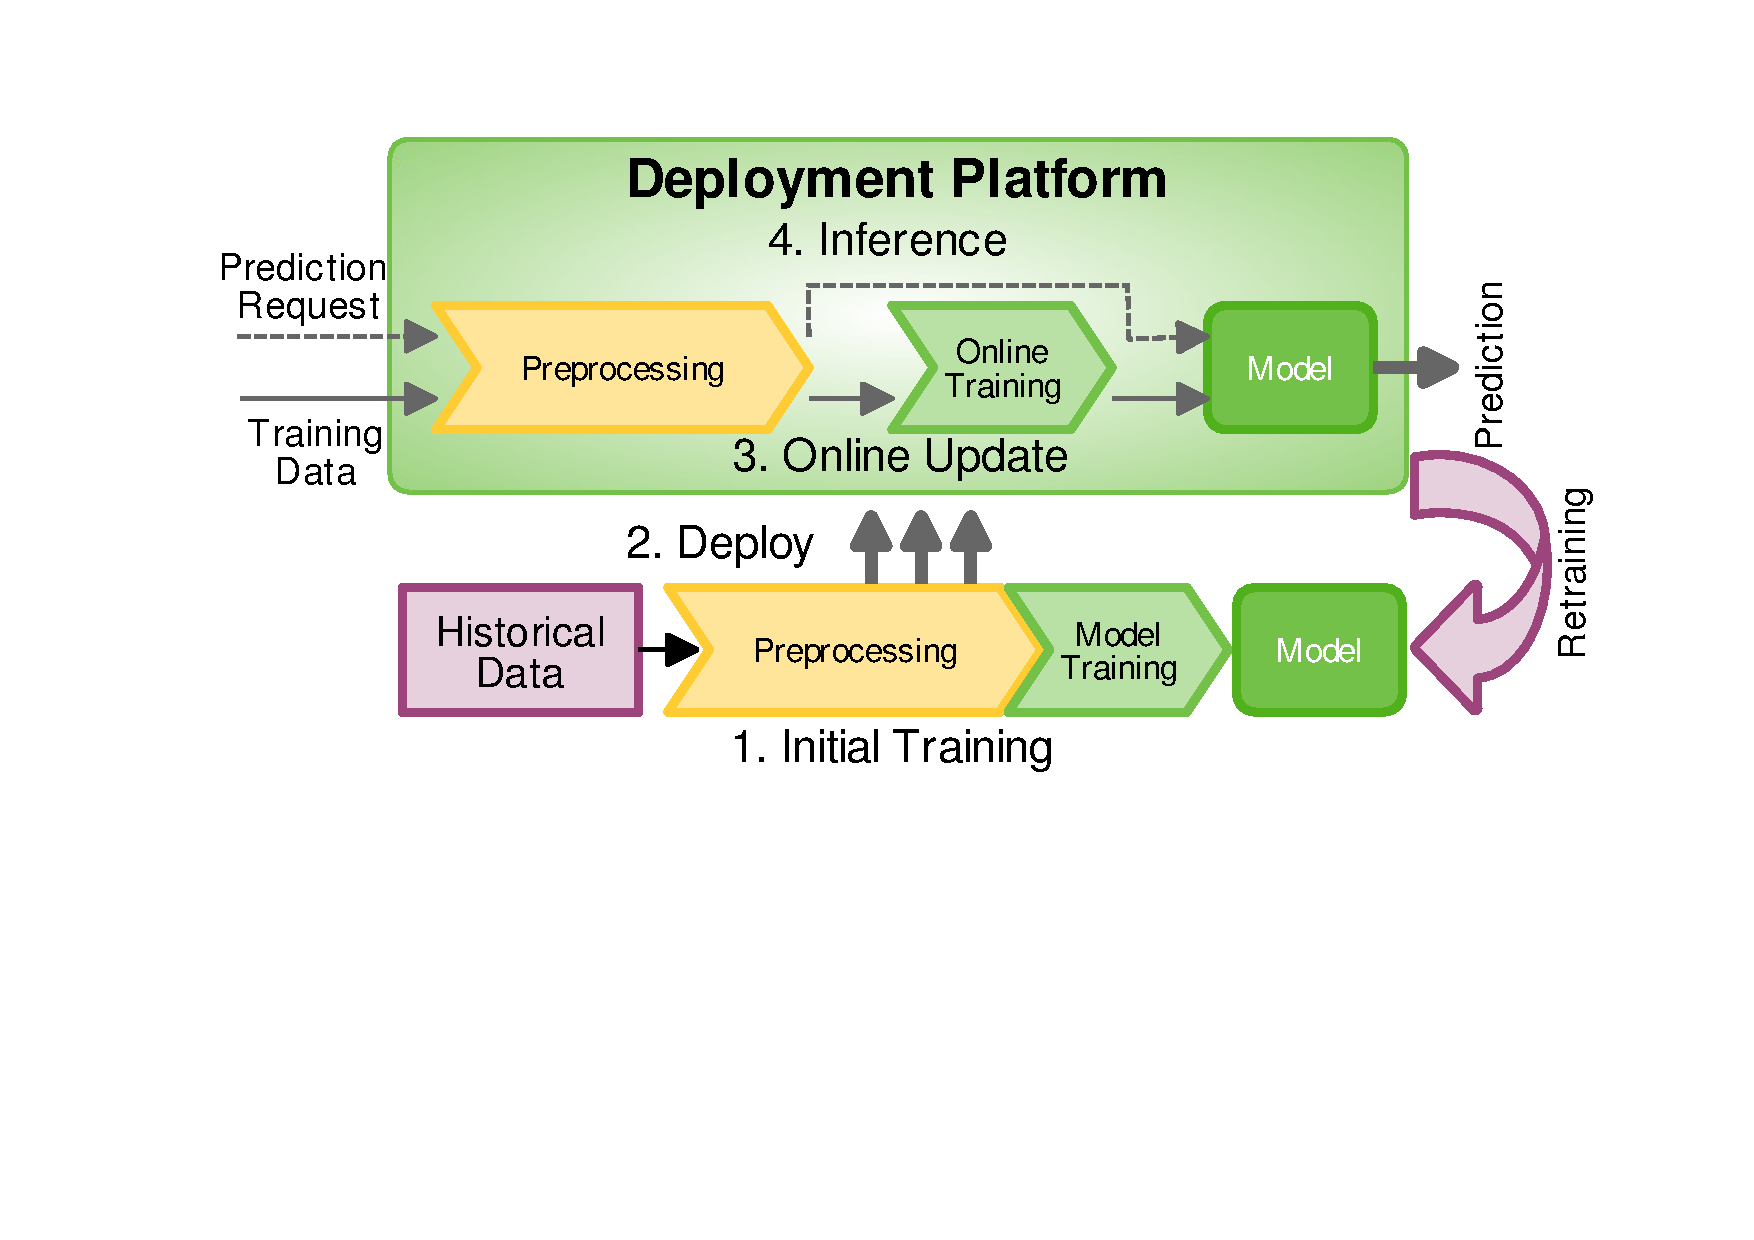
\includegraphics[width=\columnwidth]{../images/generic-motivational-example-v2.pdf}
\caption{Periodical deployment of machine learning pipelines}
\label{fig:motivational-example}
\end{subfigure}%
\begin{subfigure}{\columnwidth}
\centering
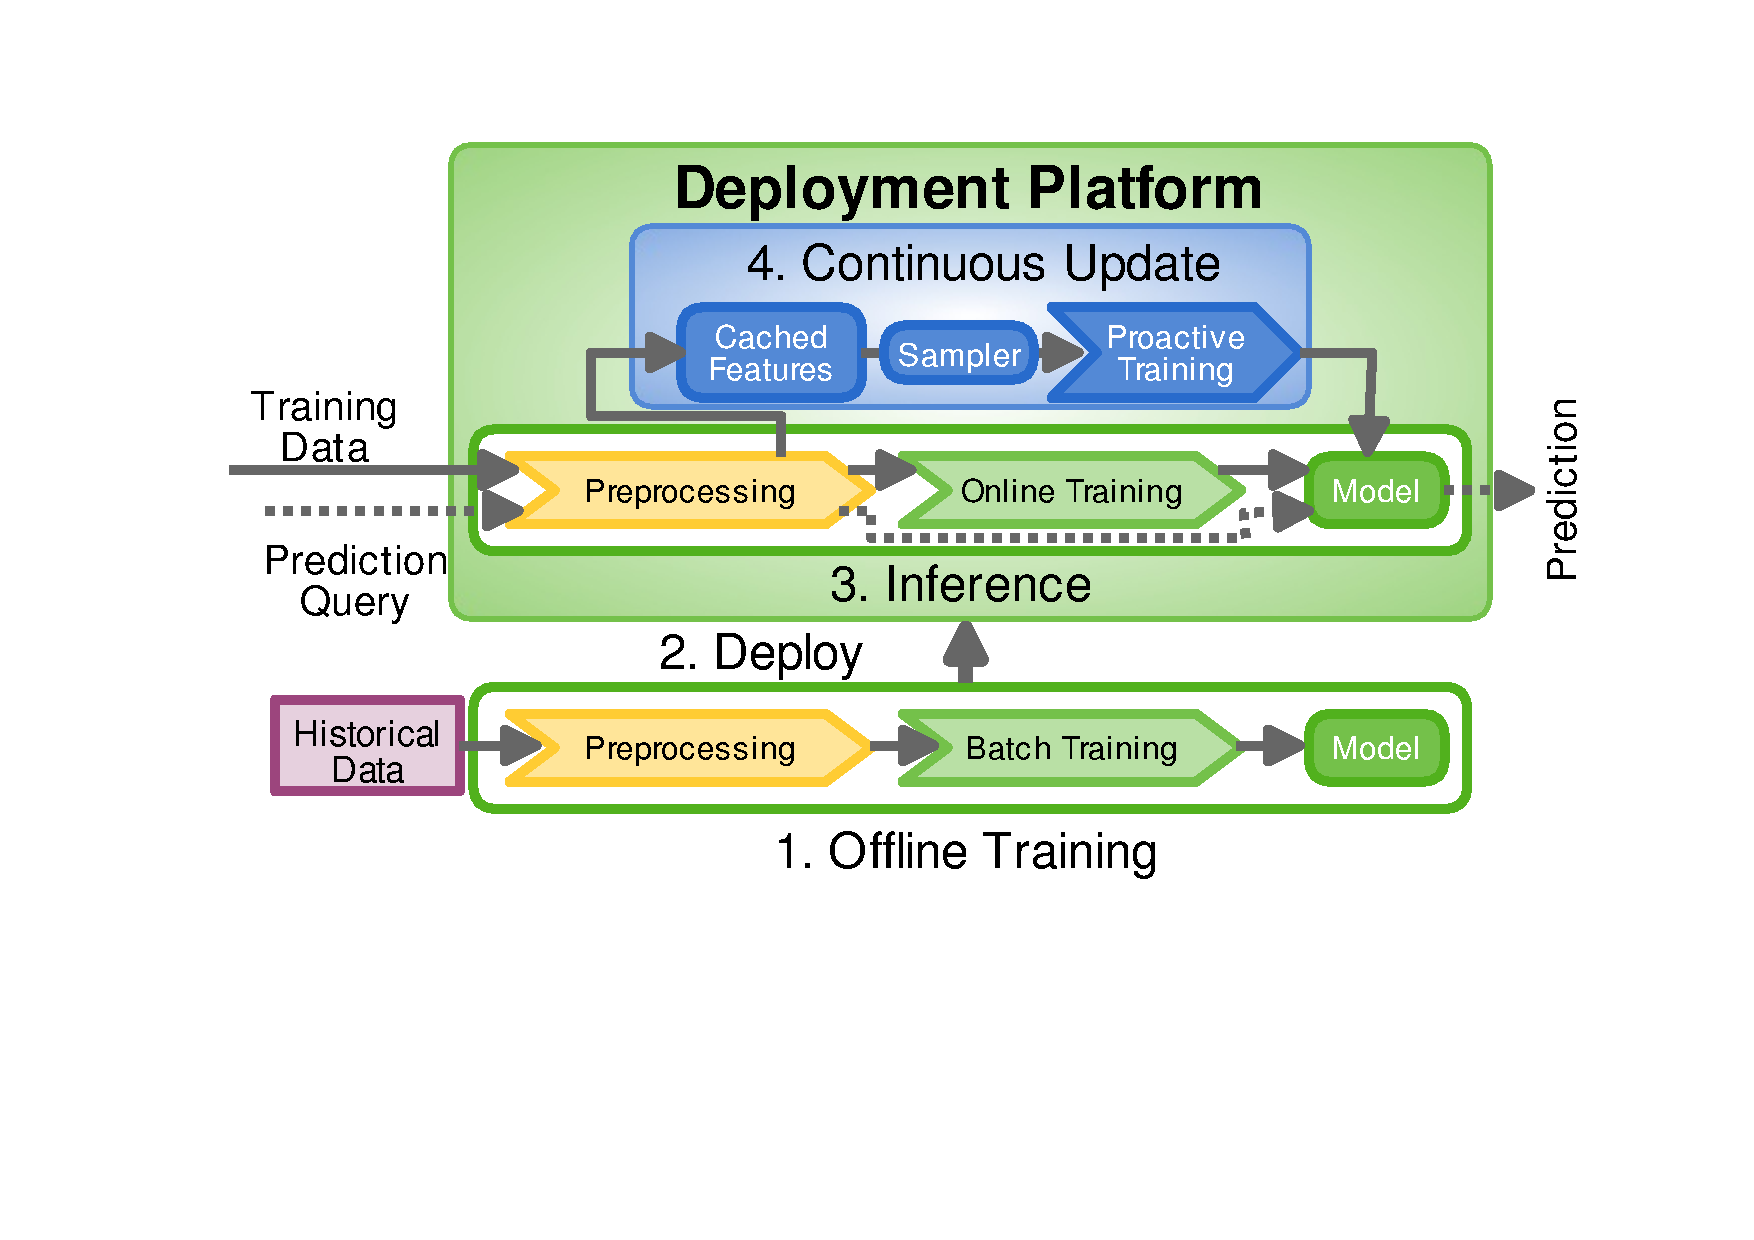
\includegraphics[width=\columnwidth]{../images/generic-improved-example-v2.pdf}
\caption{Continuous deployment of machine learning applications}
\label{fig:improved-example}
\end{subfigure}
\caption{Machine Learning Deployment Platforms}
\label{deployment-processes}
\end{figure*}
Figure \ref{deployment-processes} shows the differences in deployment processes of the periodical and continuous training approaches.
Figure \ref{fig:motivational-example} shows the process of the periodical deployment approach.
The process starts with an offline training \circled{1}.
During the offline training, a user designs a machine learning pipeline that consists of several data and feature preprocessing steps. 
After the data preprocessing step, the user trains a machine learning model by utilizing a batch training algorithm.
During the deployment step, the user deploys the model and the pipeline into the deployment platform \circled{2}.
To perform inference, the deployment platform directs the incoming prediction queries through the preprocessing steps before utilizing the model to predict the label \circled{3}.
During the online update step, the deployment platform directs the training data through the preprocessing steps of the pipeline and then, using an online training algorithm, the platform updates the model.
Finally, the deployment platform accommodates periodical retraining of the pipeline by either automatically triggering a batch training or prompting the user to train and redeploy a new model to the deployment platform \circled{4}.
During the periodical retraining, the deployment platform has to disable the online updating of the model.

Figure \ref{fig:improved-example} shows how our continuous training approach improves the existing deployment process.
Similar to the current deployment process, a user first trains a pipeline \circled{1} and deploy it into the deployment platform \circled{2}.
The deployment platform utilizes the deployed pipeline and model to answer prediction queries and update the model using the incoming training data \circled{3}.
After transforming the incoming data into a set of features, the deployment platform stores the transformed features inside a cache.
During the proactive training, the platform samples the materialized features and computes the gradient using the sample.
Finally, the platform updates the deployed model using the gradient \circled{4}.
In the new deployment approach, the platform continuously updates the pipeline and the deployed model without requiring a full retraining over the historical data.
As a result, the deployment platform ensures the model is always up-to-date.